\documentclass[]{article}
\usepackage{lmodern}
\usepackage{amssymb,amsmath}
\usepackage{ifxetex,ifluatex}
\usepackage{fixltx2e} % provides \textsubscript
\ifnum 0\ifxetex 1\fi\ifluatex 1\fi=0 % if pdftex
  \usepackage[T1]{fontenc}
  \usepackage[utf8]{inputenc}
\else % if luatex or xelatex
  \ifxetex
    \usepackage{mathspec}
  \else
    \usepackage{fontspec}
  \fi
  \defaultfontfeatures{Ligatures=TeX,Scale=MatchLowercase}
\fi
% use upquote if available, for straight quotes in verbatim environments
\IfFileExists{upquote.sty}{\usepackage{upquote}}{}
% use microtype if available
\IfFileExists{microtype.sty}{%
\usepackage{microtype}
\UseMicrotypeSet[protrusion]{basicmath} % disable protrusion for tt fonts
}{}
\usepackage[margin=1in]{geometry}
\usepackage{hyperref}
\hypersetup{unicode=true,
            pdftitle={随机模拟方法与应用导论 作业五},
            pdfauthor={陈稼霖 45875852},
            pdfborder={0 0 0},
            breaklinks=true}
\urlstyle{same}  % don't use monospace font for urls
\usepackage{color}
\usepackage{fancyvrb}
\newcommand{\VerbBar}{|}
\newcommand{\VERB}{\Verb[commandchars=\\\{\}]}
\DefineVerbatimEnvironment{Highlighting}{Verbatim}{commandchars=\\\{\}}
% Add ',fontsize=\small' for more characters per line
\usepackage{framed}
\definecolor{shadecolor}{RGB}{248,248,248}
\newenvironment{Shaded}{\begin{snugshade}}{\end{snugshade}}
\newcommand{\AlertTok}[1]{\textcolor[rgb]{0.94,0.16,0.16}{#1}}
\newcommand{\AnnotationTok}[1]{\textcolor[rgb]{0.56,0.35,0.01}{\textbf{\textit{#1}}}}
\newcommand{\AttributeTok}[1]{\textcolor[rgb]{0.77,0.63,0.00}{#1}}
\newcommand{\BaseNTok}[1]{\textcolor[rgb]{0.00,0.00,0.81}{#1}}
\newcommand{\BuiltInTok}[1]{#1}
\newcommand{\CharTok}[1]{\textcolor[rgb]{0.31,0.60,0.02}{#1}}
\newcommand{\CommentTok}[1]{\textcolor[rgb]{0.56,0.35,0.01}{\textit{#1}}}
\newcommand{\CommentVarTok}[1]{\textcolor[rgb]{0.56,0.35,0.01}{\textbf{\textit{#1}}}}
\newcommand{\ConstantTok}[1]{\textcolor[rgb]{0.00,0.00,0.00}{#1}}
\newcommand{\ControlFlowTok}[1]{\textcolor[rgb]{0.13,0.29,0.53}{\textbf{#1}}}
\newcommand{\DataTypeTok}[1]{\textcolor[rgb]{0.13,0.29,0.53}{#1}}
\newcommand{\DecValTok}[1]{\textcolor[rgb]{0.00,0.00,0.81}{#1}}
\newcommand{\DocumentationTok}[1]{\textcolor[rgb]{0.56,0.35,0.01}{\textbf{\textit{#1}}}}
\newcommand{\ErrorTok}[1]{\textcolor[rgb]{0.64,0.00,0.00}{\textbf{#1}}}
\newcommand{\ExtensionTok}[1]{#1}
\newcommand{\FloatTok}[1]{\textcolor[rgb]{0.00,0.00,0.81}{#1}}
\newcommand{\FunctionTok}[1]{\textcolor[rgb]{0.00,0.00,0.00}{#1}}
\newcommand{\ImportTok}[1]{#1}
\newcommand{\InformationTok}[1]{\textcolor[rgb]{0.56,0.35,0.01}{\textbf{\textit{#1}}}}
\newcommand{\KeywordTok}[1]{\textcolor[rgb]{0.13,0.29,0.53}{\textbf{#1}}}
\newcommand{\NormalTok}[1]{#1}
\newcommand{\OperatorTok}[1]{\textcolor[rgb]{0.81,0.36,0.00}{\textbf{#1}}}
\newcommand{\OtherTok}[1]{\textcolor[rgb]{0.56,0.35,0.01}{#1}}
\newcommand{\PreprocessorTok}[1]{\textcolor[rgb]{0.56,0.35,0.01}{\textit{#1}}}
\newcommand{\RegionMarkerTok}[1]{#1}
\newcommand{\SpecialCharTok}[1]{\textcolor[rgb]{0.00,0.00,0.00}{#1}}
\newcommand{\SpecialStringTok}[1]{\textcolor[rgb]{0.31,0.60,0.02}{#1}}
\newcommand{\StringTok}[1]{\textcolor[rgb]{0.31,0.60,0.02}{#1}}
\newcommand{\VariableTok}[1]{\textcolor[rgb]{0.00,0.00,0.00}{#1}}
\newcommand{\VerbatimStringTok}[1]{\textcolor[rgb]{0.31,0.60,0.02}{#1}}
\newcommand{\WarningTok}[1]{\textcolor[rgb]{0.56,0.35,0.01}{\textbf{\textit{#1}}}}
\usepackage{graphicx,grffile}
\makeatletter
\def\maxwidth{\ifdim\Gin@nat@width>\linewidth\linewidth\else\Gin@nat@width\fi}
\def\maxheight{\ifdim\Gin@nat@height>\textheight\textheight\else\Gin@nat@height\fi}
\makeatother
% Scale images if necessary, so that they will not overflow the page
% margins by default, and it is still possible to overwrite the defaults
% using explicit options in \includegraphics[width, height, ...]{}
\setkeys{Gin}{width=\maxwidth,height=\maxheight,keepaspectratio}
\IfFileExists{parskip.sty}{%
\usepackage{parskip}
}{% else
\setlength{\parindent}{0pt}
\setlength{\parskip}{6pt plus 2pt minus 1pt}
}
\setlength{\emergencystretch}{3em}  % prevent overfull lines
\providecommand{\tightlist}{%
  \setlength{\itemsep}{0pt}\setlength{\parskip}{0pt}}
\setcounter{secnumdepth}{0}
% Redefines (sub)paragraphs to behave more like sections
\ifx\paragraph\undefined\else
\let\oldparagraph\paragraph
\renewcommand{\paragraph}[1]{\oldparagraph{#1}\mbox{}}
\fi
\ifx\subparagraph\undefined\else
\let\oldsubparagraph\subparagraph
\renewcommand{\subparagraph}[1]{\oldsubparagraph{#1}\mbox{}}
\fi

%%% Use protect on footnotes to avoid problems with footnotes in titles
\let\rmarkdownfootnote\footnote%
\def\footnote{\protect\rmarkdownfootnote}

%%% Change title format to be more compact
\usepackage{titling}

% Create subtitle command for use in maketitle
\providecommand{\subtitle}[1]{
  \posttitle{
    \begin{center}\large#1\end{center}
    }
}

\setlength{\droptitle}{-2em}

  \title{随机模拟方法与应用导论 作业五}
    \pretitle{\vspace{\droptitle}\centering\huge}
  \posttitle{\par}
    \author{陈稼霖 45875852}
    \preauthor{\centering\large\emph}
  \postauthor{\par}
      \predate{\centering\large\emph}
  \postdate{\par}
    \date{2019-10-03}

\usepackage[UTF8]{ctex}

\begin{document}
\maketitle

\hypertarget{exploring-percentages-of-full-time-faculty}{%
\section{5.5 (Exploring percentages of full-time
faculty)}\label{exploring-percentages-of-full-time-faculty}}

The variable \texttt{Full.time} in the college dataset (see Example 5.3)
contains the percentage of faculty who are hired full-time in the group
of National Universities.

\begin{enumerate}
\def\labelenumi{\alph{enumi}.}
\item
  Using the \texttt{hist} function, construct a histogram of the
  full-time percentages and comment on the shape of the distribution.
\item
  Use the froot and flog transformations to reexpress the full-time
  percentages. Construct histograms of the collection of froots and the
  collection of flogs. Is either transformation successful in making the
  full-time percentages approximately symmetric?
\item
  For data that is approximately normally distributed, about \(68\%\) of
  the data fall within one standard deviation of the mean. Assuming you
  have found a transformation in part (b) that makes the full-time
  percentages approximately normal, find an interval that contains
  roughly \(68\%\) of the data on the new scale.
\end{enumerate}

\begin{enumerate}
\def\labelenumi{\alph{enumi}.}
\tightlist
\item
  首先读取文件\texttt{college.txt}
\end{enumerate}

\begin{Shaded}
\begin{Highlighting}[]
\NormalTok{dat =}\StringTok{ }\KeywordTok{read.table}\NormalTok{(}\StringTok{'college.txt'}\NormalTok{,}\DataTypeTok{head =} \OtherTok{TRUE}\NormalTok{,}\DataTypeTok{sep =} \StringTok{'}\CharTok{\textbackslash{}t}\StringTok{'}\NormalTok{)}
\end{Highlighting}
\end{Shaded}

然后依据变量\texttt{Full.time}绘制全职教职工百分比的直方图

\begin{Shaded}
\begin{Highlighting}[]
\KeywordTok{hist}\NormalTok{(dat}\OperatorTok{$}\NormalTok{Full.time,}\DataTypeTok{xlab =} \StringTok{'Full-time Faculty Percentage'}\NormalTok{,}
     \DataTypeTok{main =} \StringTok{'Full-time Faculty Percentage'}\NormalTok{)}
\end{Highlighting}
\end{Shaded}

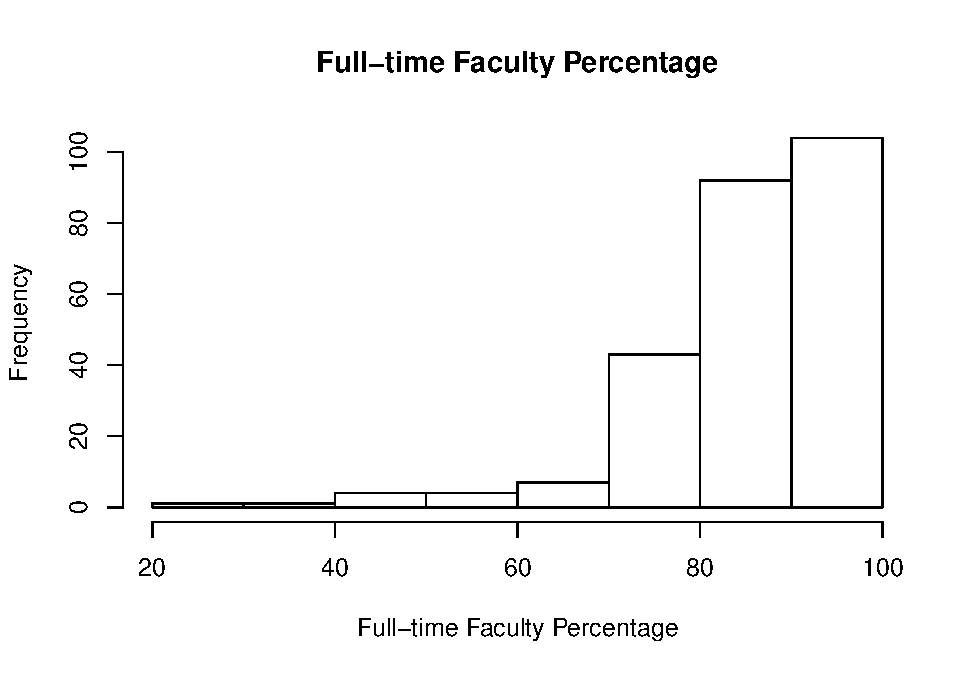
\includegraphics{Homework_5_files/figure-latex/unnamed-chunk-2-1.pdf}

评价:由图可见,绝大多数大学的全职教职工百分比在\(80\%\)以上,直方图形状右偏(right-skewed)。

\begin{enumerate}
\def\labelenumi{\alph{enumi}.}
\setcounter{enumi}{1}
\tightlist
\item
  用froot转换重新表示全职教职工百分比并绘制其直方图
\end{enumerate}

\begin{Shaded}
\begin{Highlighting}[]
\NormalTok{froot =}\StringTok{ }\KeywordTok{sqrt}\NormalTok{(dat}\OperatorTok{$}\NormalTok{Full.time) }\OperatorTok{-}\StringTok{ }\KeywordTok{sqrt}\NormalTok{(}\DecValTok{100} \OperatorTok{-}\StringTok{ }\NormalTok{dat}\OperatorTok{$}\NormalTok{Full.time)}
\KeywordTok{hist}\NormalTok{(froot,}\DataTypeTok{xlab =} \StringTok{'Full-time Faculty Percentage(froot)'}\NormalTok{,}
     \DataTypeTok{main =} \StringTok{'Full-time Faculty Percentage (froot) histogram'}\NormalTok{)}
\end{Highlighting}
\end{Shaded}

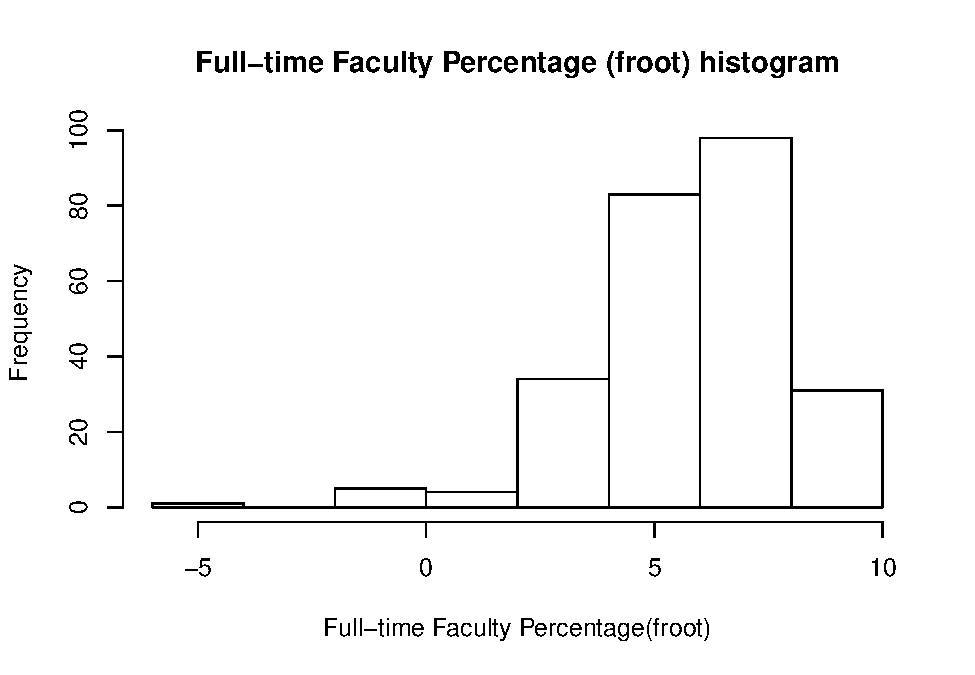
\includegraphics{Homework_5_files/figure-latex/unnamed-chunk-3-1.pdf}

用flog转换重新表示全职教职工百分比并绘制其分布直方图

\begin{Shaded}
\begin{Highlighting}[]
\NormalTok{flog =}\StringTok{ }\KeywordTok{log}\NormalTok{(dat}\OperatorTok{$}\NormalTok{Full.time) }\OperatorTok{-}\StringTok{ }\KeywordTok{log}\NormalTok{(}\DecValTok{100} \OperatorTok{-}\StringTok{ }\NormalTok{dat}\OperatorTok{$}\NormalTok{Full.time)}
\KeywordTok{hist}\NormalTok{(flog,}\DataTypeTok{xlab =} \StringTok{'Full-time Faculty Percentage (flog)'}\NormalTok{,}
     \DataTypeTok{main =} \StringTok{'Full-time Faculty Percentage (flog) histogram'}\NormalTok{)}
\end{Highlighting}
\end{Shaded}

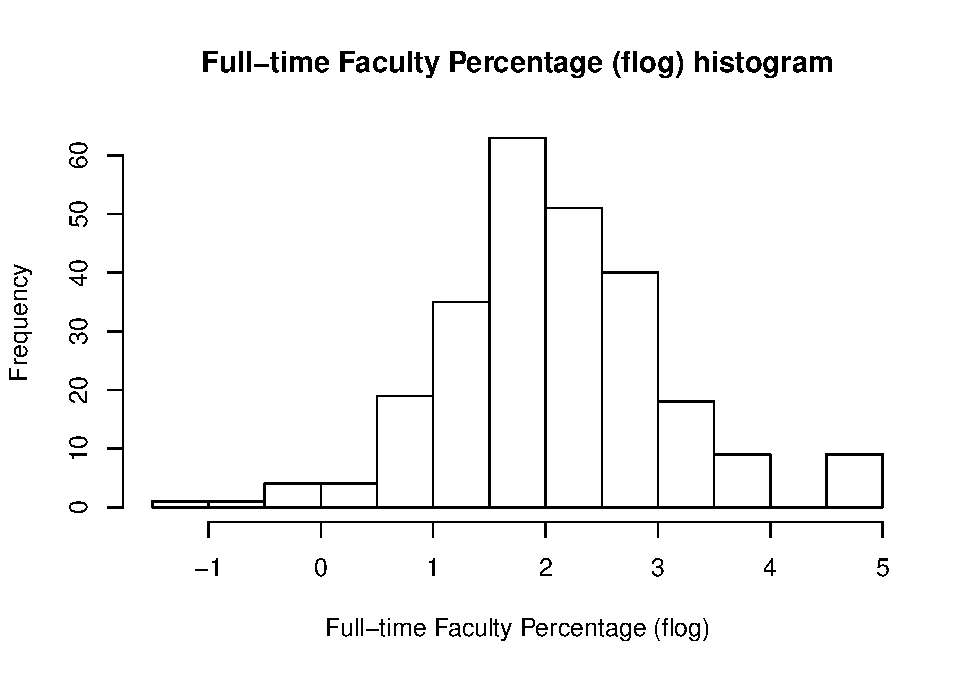
\includegraphics{Homework_5_files/figure-latex/unnamed-chunk-4-1.pdf}

两种转换都使得全职教职工百分比的直方图更加对称。

\begin{enumerate}
\def\labelenumi{\alph{enumi}.}
\setcounter{enumi}{2}
\tightlist
\item
  对于froot转换后得到的直方图,约\(68\%\)的数据集中的区间为\((4,8]\);对于flog转换后得到的直方图,约\(68\%\)的数据集中的区间为\((1,3]\)。
\end{enumerate}


\end{document}
